\section{Kaka Kamaludin}
\subsection{Teori}

\begin{enumerate}
	\item Definisi, Sejarah dan Perkembangan Kecerdasan Buatan

		\begin{itemize}
			\item Definisi Kecerdasan Buatan
				\paragraph{}
				Kecerdasan Buatan biasa disebut dengan istilah AI (Artificial Intelligence). AI sendiri merupakan suatu cabang dalam bisnis sains komputer sains dimana mengkaji tentang bagaimana cara untuk menlengkapi sebuah komputer dengan kemampuan atau kepintaran layaknya atau mirip dengan yang dimiliki manusia. Sebagai contoh, sebagaimana komputer dapat berkomunikasi dengan pengguna baik menggunakan kata, suara maupun lain sebagainya. Dengan kemampuan ini, diharapkan komputer mampu mengambil keputusan sendiri untuk berbagai kasus yang ditemuinya kemudian itulah yang disebut dengan kecerdasan buatan. 
				\paragraph{}
				Kecerdasan Buatan adalah salah satu bidang studi yang berhubungan dengan pemanfaatan mesin untuk memecahkan persoalan yang rumit dengan cara lebih manusiawi dan lebih bisa di pahami oleh manusia. Kecerdasan buatan makin canggih dengan kemampuan komputer dalam memperbarui pengetahuannya dengan testing dan perkembangan target analisa.
			
			\item Sejarah Kecerdasan Buatan
				\paragraph{}
				Pada tahun 1956, McCarthy yang sama mendirikan Konferensi Dartmouth di Hanover, New Hampshire. Peneliti terkemuka dalam teori kompleksitas, simulasi bahasa, hubungan antara keacakan dan pemikiran kreatif, jaringan saraf diundang. Tujuan dari bidang penelitian yang baru dibuat adalah untuk mengembangkan mesin yang dapat mensimulasikan setiap aspek kecerdasab. Itulah sebabnya Konferensi Dartmouth 1956 dianggap sebagai kelahiran Kecerdasan Buatan. Sejak saat itu, Kecerdasa Buatan telah hidup melalui decade kemuliaan dan cemoohan, yang dikenal luas sebagai musim panas dan musim dingin AI. Musim panasnya ditandai dengan optimism dan dana besar, sedangkan musim dinginnya dihadapkan dengan pemotongan dana, ketidakkpercayaan dan pesimisme.
				
				 \paragraph{}
				Artificial intelligence merupakan inovasi baru di bidang ilmu pengetahuan. Mulai terbentuk sejak adanya komputer modern dan kira-kira terjadi sekitaran tahun 1940 dan 1950. Ilmu pengetahuan komputer ini khusus ditujukan dalam perancangan otomatisasi tingkah laku cerdas dalam sistem kecerdasan komputer. Pada awal 50-an, studi tentang “mesin berpikir” memiliki berbagai nama seperti cybernetics, teori automata, dan pemrosesan innformasi. Pada tahun 1956, para ilmuan jenius seperti Alan Turing, Norbert, Wiener, Claude Shannon dan Warren McCullough telah bekerja secara independen dibidang cybernetics, matematika, algoritma dan teori jaringan. Namun, seprang ilmuan komputer dan kognitif John McCarthy adalah orang yang dating dengan ide untuk bergabung dengan upaya penelitian terpisah ini kedalam satu bidang yang akan mempelajari topic baru untuk imajinasi manusia yaitu kecerdasan buatan. Dia adalah orang yang menciptakan istilah tersebut dan kemudian mendirikan laboratorium Kecerdasan Buatan di MIT dan Stan
				ford.
				
			\item Perkembangan Kecerdasan Buatan
			
				\paragraph{}
				Teknologi Artificial Intelligence semakin ramai dibahas dalam berbagai diskusi teknologi di seluruh dunia.Menurut kebanyakan orang, pekerjaan seperti kasir, operator telepon, pengendara truk, dan lainnya sangat berpeluang besar untuk tergantikan oleh Artificial Intelligence. Mengapa terjadi hal demikian? dikarenakan memang bahwa AI lebih ungul dalam hal kinerja, fitur dan lain sebagainya. Namun, dalam beberapa aspek memang pekerja manusia masih unggul dibandingkan AI itu sendiri. Para generasi muda yang ada di dunia terutama di daerah Asia terlihat sudah memahami fungsi dan efek dari AI dalam kehidupan kita sehari-hari. Berdasarkan survei yang dilakukan oleh Microsoft, terdapat 39 persen responden yang mempertimbangkan untuk menggunakan mobil tanpa pengemudi dan 36 persen lainnya setuju bahwa robot masa depan dengan software untuk beroperasi mampu meningkatkan produktivitas. Dari survey tersebut kita sebagai pengguna AI harus lebih bijaksana dalam pengembangan dan penggunaan dari AI sehingga tanpa memberikan efek samping terhadap etos kerja dan keseharian kita sebagai pengguna dalam kehidupan seharihari.
				
				\paragraph{}
				AI Summer 1 (1956-1973) KOnferensi Dartmounth diikuti oleh 17 tahun kemajuan luar biasa. Proyek penelitian yang dilakukan di MIT, universitas di Edinburgh, Stanford dan Carnegie Mellon menerima dana besar-besaran, yang akhirnya membuahkan hasil. Selama tahun-tahun itulah komputer pemrograman mulai melakukan masalah aljabar, membuktikan teorema geometris, memahami dan menggunakan sintaks dan tata bahasa Inggris. Terlepas dari ditinggalkannya koneksionisme dan terjemahan mesin yang gagal, yang menunda penelitian Natural Language Processing (NLP) selama bertahun-tahun, banyak prestasi dari masa lalu yang membuat sejarah. Berikut ini beberapa diantaranya : Pelopor pembelajaran mesin, Ray Solomonoff meletakkan dasar-dasar teori metematika AI, memperkenalkan metode Bayesian universal untuk inferensi dan preddiksi induktif Thomas Evans menciptakan program ANALOGI heuristik, yang memungkinkan komputer memecahkan masalah geometrianalogi Unimation, perusahaan robotika pertma didunia, menciptakan robot industri Unimate, yang bekerja pada jalur perakitan modil Genenral Motors. Joseph Weizenbaum membangun ELIZA-program interaktif yang dapat membawa percakapan dalam bahasan Inggris tentang topik apapun. Ross Quillian menunjukkan jaring semanik, sedangkan Jaime Carbonell (Sr.) mengembangkan Cendikia-program interaktif untuk instruksi yang dibantu komputer berdasarkan jaring semantik. Edward Feigenbaum dan Julian Feldman menerbitkan Computeks and Thought, kumpulan artikel pertama tentang AI.
				
		\end{itemize}
		
	\item Definisi Supervised Learning, Klasifikasi, Regresi, Unsupervised Learning, Data Set, Training Set dan Testing Set
		
		\begin{itemize}
			\item Definisi Supervised Learning
				\paragraph{}
				Supervised Learning adalah tugas pengumpulan data untuk menyimpulkan fungsi dari data pelatihan berlabel. Data pelatihan terdiri dari serangkaian contoh pelatihan. Dalam supervised learning, setiap contoh adalah pasangan yang terdiri dari objek input (biasanya vektor) dan nilai output yang diinginkan(juga disebut sinyal pengawasan super). Algoritma pembelajaran yang diawasi menganalisis data pelatihan dan menghasilkan fungsi yang disimpulkan, yang dapat digunakan untuk memetakan contoh-contoh baru. Skenario optimal akan memungkinkan algoritma menentukan label kelas dengan benar untuk instance yang tidak terlihat. Ini membutuhkan algoritma pembelajaran untuk menggeneralisasi dari data pelatihan untuk situasi yang tidak terlihat dengan cara yang ”masuk akal”. Supervised Learning menyediakan algoritma pembelajaran dengan jumlah yang diketahui untuk mendukung penilaian dimasa depan. Chatbots, mobil self-driving, program pengenalan wajah, sistem pakar dan robot adalah beberapa sistem yang dapat menggunakan pembelajaran yang diawasi atau tidak diawasi. Supervised Learning sebagian besar terkait dengan AI berbasis pengambilan tetapi mereka juga mungkin mampu menggunakan model pembelajaran generatif. Data pelatihan untuk pembelajaran yang diawasi mencakup serangkaian contoh dengan subjek input berpasangan dan output yang diinginkan (yang juga disebut sebagai sinyal pengawasan).
			
			\item Klasifikasi
				\paragraph{}
				Klasifikasi adalah pembagian sesuatu menurut kelas-kelas ( class ). Menurut Ilmu Pengetahuan, Klasifikasi merupakan proses pengelompokkan benda berdasarkan ciriciri persamaan dan juga perbedaan. Dalam masalah klasifikasi, kami mencoba memprediksi sejumlah nilai terpisah. Label (y) umumnya datang dalam bentuk kategorikal dan mewakili sejumlah kelas. Dalam pembelajaran mesin dan statistik, klasifikasi adalah pendekatan pembelajaran yang diawasi di mana program komputer belajar dari input data yang diberikan kepadanya dan kemudian menggunakan pembelajaran ini untuk mengklasifikasikan pengamatan baru. Kumpulan data ini mungkin hanya bersifat dua kelas (seperti mengidentifikasi apakah orang tersebut berjenis kelamin laki-laki atau perempuan atau bahwa surat itu spam atau bukan-spam) atau mungkin juga multi-kelas. Beberapa contoh masalah klasifikasi adalah: pengenalan ucapan, pengenalan tulisan tangan, identifikasi metrik, klasifikasi dokumen dll.

			\item Regresi
				\paragraph{}
				Regresi adalah metode analisis statistik yang digunakan untuk melihat pengaruh antara dua ataupun lebih variabel. Regresi adalah membahas masalah ketika variabel output adalah nilai riil atau berkelanjutan, seperti ”gaji” atau ”berat”. Banyak model yang berbeda dapat digunakan makan, yang paling sederhana adalah regresi linier. Ia mencoba untuk menyesuaikan data dengan hyper-plane terbaik yang melewati poin.
				
			\item Unsupervised Learning
				\paragraph{}
				Unsupervised Learning adalah pelatihan algoritma kecerdasan buatan (AI) menggunakan informasi yang tidak diklasifikasikan atau diberi label dan memungkinkan algoritma untuk bertindak atas informasi tersebut tanpa bimbingan. Dalam Unsupervised Learning, sistem AI dapat mengelompokkan informasi yang tidak disortir berdasarkan persamaan dan perbedaan meskipun tidak ada kategori yang disediakan.
				
			\item Data set
				\paragraph{}
				Dataset adalah objek yang merepresentasikan data dan juga relasi yang ada di memory. Strukturnya mirip dengan data di database, namun bedanya dataset berisi koleksi dari data table dan data relation. mendapatkan data yang tepat berarti mengumpulkan atau mengidentifikasi data yang berkorelasi dengan hasil yang ingin Anda prediksi; yaitu data yang berisi sinyal tentang peristiwa yang Anda pedulikan. Data harus diselaraskan dengan masalah yang Anda coba selesaikan. Gambar kucing tidak terlalu berguna ketika Anda sedang membangun sistem identifikasi wajah. Memverifikasi bahwa data selaras dengan masalah yang ingin Anda selesaikan harus dilakukan oleh ilmuwan data. Jika Anda tidak memiliki data yang tepat, maka upaya Anda untuk membangun solusi AI harus kembali ke tahap pengumpulan data.

			\item Training Set
				\paragraph{}
				Training Set adalah set digunakan oleh algoritma klassifikasi . Dapat dicontohkan dengan : decision tree, bayesian, neural network dll. Semuanya dapat digunakan untuk membentuk sebuah model classifier. Menjalankan pelatihan yang diatur melalui jaringan saraf mengajarkan pada net cara menimbang berbagai fitur, menyesuaikan koefisien berdasarkan kemungkinan mereka meminimalkan kesalahan dalam hasil Anda. Koefisien-koefisien tersebut, juga dikenal sebagai parameter, akan terkandung dalam tensor dan bersama-sama mereka disebut model, karena mereka mengkodekan model data yang mereka latih. Mereka adalah takeaways paling penting yang akan Anda dapatkan dari pelatihan jaringan saraf.

			\item Testing set
				\paragraph{}
				Testing Set adalah set yang digunakan untuk mengukur sejauh mana classifier berhasil melakukan klasifikasi dengan benar. Ini berfungsi sebagai meterai persetujuan, dan Anda tidak menggunakannya sampai akhir. Setelah Anda melatih dan mengoptimalkan data Anda, Anda menguji jaringan saraf Anda terhadap pengambilan sampel acak akhir ini. Hasil yang dihasilkannya harus memvalidasi bahwa jaring Anda secara akurat mengenali gambar, atau mengenalinya setidaknya [x] dari jumlah tersebut. Jika Anda tidak mendapatkan prediksi yang akurat, kembalilah ke set pelatihan,
				lihat hyperparameter yang Anda gunakan untuk menyetel jaringan, serta kualitas data Anda dan lihat teknik pra-pemrosesan Anda.
				
		\end{itemize}
		
\end{enumerate}


\subsection{Praktek}

	\begin{enumerate}
		\item Instalasi library scikit dari anaconda, mencoba kompilasi dan uji coba ambil contoh kode dan lihat variabel explorer

			\begin{itemize}
				\item Buka promt anaconda lalu ketikkan conda scikit-learn
				\item Biarkan proses berjalan hingga selesai
			\end{itemize}
		
			\begin{figure}[H]
				\begin{center}
				 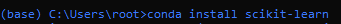
\includegraphics[width=10cm]{figures/1174067/1/1.png}
				 \caption{Install library scikit}	
				\end{center}
			\end{figure}
			
			\begin{figure}[H]
				\begin{center}
				 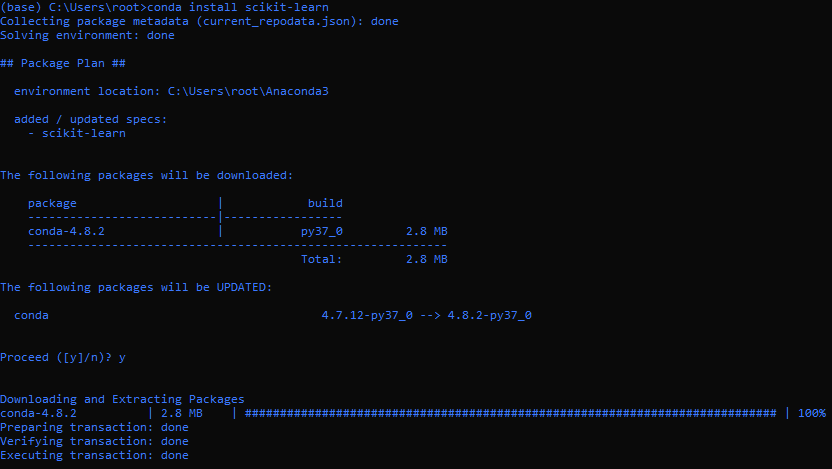
\includegraphics[width=10cm]{figures/1174067/1/2.png}
				 \caption{Proses jika berhasil}	
				\end{center}
			\end{figure}
	
		\item Mencoba Loading an example dataset, menjelaskan maksud dari tulisan tersebut dan mengartikan per baris

			\begin{itemize}
				\item Ketikkan script berikut di spyder, lalu run
				\lstinputlisting[firstline=1, lastline=11]{src/1174067/1/test.py}	
			\end{itemize}

			\begin{figure}[H]
				\begin{center}
				 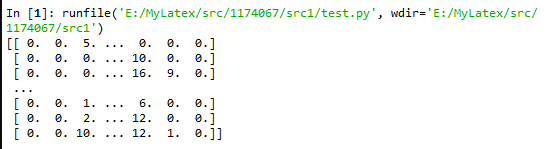
\includegraphics[width=10cm]{figures/1174067/1/3.png}
				 \caption{hasil test.py}	
				\end{center}
			\end{figure}

		\item Mencoba Learning and predicting, menjelaskan maksud dari tulisan tersebut dan mengartikan perbaris	
			\lstinputlisting[firstline=1, lastline=24]{src/1174067/1/test2.py}

			\begin{figure}[H]
				\begin{center}
				 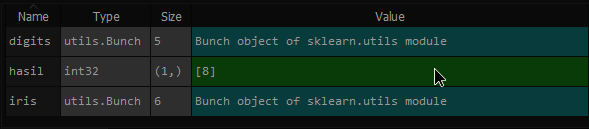
\includegraphics[width=10cm]{figures/1174067/1/test2.png}
				 \caption{variabel explorer test2.py}	
				\end{center}
			\end{figure}
			
			
		\item Mencoba Model persistence, menjelaskan maksud dari tulisan tersebut dan mengartikan per baris
			\lstinputlisting[firstline=1, lastline=63]{src/1174067/1/test3.py}			
	
			\begin{figure}[H]
				\begin{center}
				 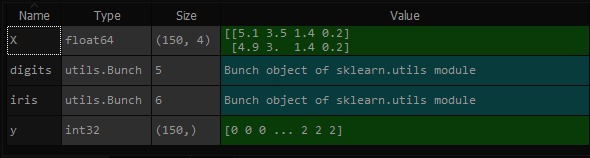
\includegraphics[width=10cm]{figures/1174067/1/test3.png}
				 \caption{variabel explorer test3.py}	
				\end{center}
			\end{figure}
			
	
		\item Mencoba Conventions, menjelaskan maksud dari tulisan tersebut dan mengartikan per baris
			\lstinputlisting[firstline=1, lastline=27]{src/1174067/1/test4.py}			
	
			\begin{figure}[H]
				\begin{center}
				 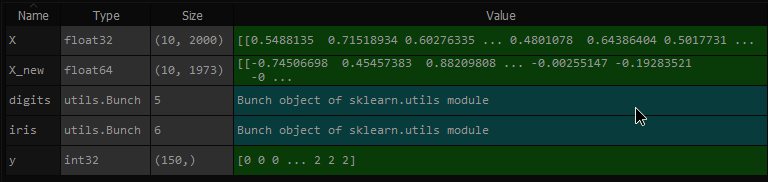
\includegraphics[width=10cm]{figures/1174067/1/test4ve.png}
				 \caption{variabel explorer test4.py}	
				\end{center}
			\end{figure}
			
			\begin{figure}[H]
				\begin{center}
				 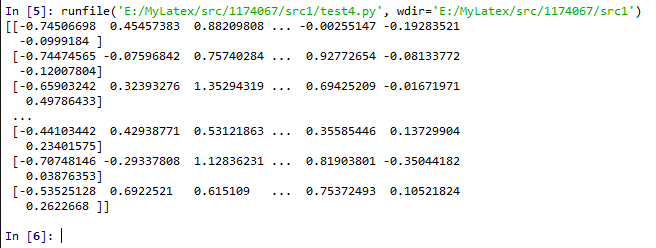
\includegraphics[width=10cm]{figures/1174067/1/test4.png}
				 \caption{hasil test4.py}	
				\end{center}
			\end{figure}
	
	\end{enumerate}
	

\subsection{Penanganan Error}

	\begin{enumerate}
		\item Screenshoots Error
			\begin{figure}[H]
				\begin{center}
				 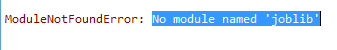
\includegraphics[width=10cm]{figures/1174067/1/error_1.png}
				 \caption{error}	
				\end{center}
			\end{figure}
			
		\item Jenis Error
			\begin{itemize}
				\item Not Module name "joblib"
			\end{itemize}
			
			\item Cara Penanganan Error
			\begin{itemize}
				\item install library joblib
			\end{itemize}
			
	\end{enumerate}
	
\subsection{Bukti tidak plagiat}

\subsection{Link Youtube}
https://youtu.be/FDQopV2LUIo
	